\documentclass[conference, 11pt]{IEEEtran}
\IEEEoverridecommandlockouts

\usepackage{algorithm}
\usepackage{algpseudocode}
\usepackage{multirow}
\usepackage{multicol}
\usepackage{siunitx}
\usepackage{booktabs}
\usepackage{listings}
\usepackage{stfloats}
\usepackage{midfloat}
\usepackage{color}
\usepackage[table]{xcolor}
\usepackage{lipsum}
\usepackage[utf8x]{inputenc}

\usepackage{bbm}
\usepackage{graphicx}
\usepackage{amsmath}
\usepackage[colorlinks=true,linkcolor=black,anchorcolor=black,citecolor=black,filecolor=black,menucolor=black,runcolor=black,urlcolor=black]{hyperref}

\newtheorem{thm}{Theorem}[section]
\newtheorem{defn}[thm]{Def.}
\newtheorem{propen}[thm]{Prop.}
\newtheorem{cor}[thm]{Cor.}

\def\BibTeX{{\rm B\kern-.05em{\sc i\kern-.025em b}\kern-.08em
		T\kern-.1667em\lower.7ex\hbox{E}\kern-.125emX}}

\title{Advanced Methods for Autonomous Driving based on Adaptive Model Predictive Control}
\author{\IEEEauthorblockN{Alberto Franco}\\
\IEEEauthorblockA{Department of Information Engineering\\
Università degli Studi di Padova\\ \href{mailto:alberto.franco.3@studenti.unipd.it}{alberto.franco.3@studenti.unipd.it}}}

\begin{document}
\maketitle
\begin{abstract}
	In this paper we present two different strategies for a self-driving car. The aim of this project is to study and implement a path tracking framework in order to prevent ATLASCAR2 collision with moving obstacle vehicles. The proposed algorithms, based on the Model Predictive Control paradigm, solve optimal problems formulated in terms of cost minimization under constraints.
\end{abstract}

\section{Introduction}
In robotic research, the problem of navigation is among the most important. Basically all autonomous mobile robots need some kind of navigation to fulfill the mobile term.
We understand navigation as a process of planning a path of a mobile robot from its current position to a desired goal location, following the planned path, and avoiding any discovered obstacles along the way. The desired paths have to
fulfill several conditions to ensure safety and feasibility of the navigation. Moreover, the paths can be also compared in terms of desirability for example short or smooth paths are usually more desirable than long and curved ones. Such paths should therefore be preferred in the navigation process. Beyond the path planning, the navigation problem also involves reacting to changes of the environment model. Robots are required to move towards target in a short time and avoid either static or dynamic obstacles observed by their sensors, which involves efficient path planning and valid obstacle avoidance. Though these two topics have been well researched, currently, there is no ideal solution to handling the navigation problem within cluttered dynamic environments.

\section{Context of the Problem and \\  Proposed Solution}
The ATLACAR2 has a sensor, such as lidar, that measures the distance to an obstacle in front of the vehicle and in the same lane. The obstacle can be static, such as a large pothole, or moving, such as a slow-moving vehicle. The most common maneuver from the driver is to temporarily move to another lane, drive past the obstacle, and move back to the original lane afterward.
In this case, we want to design an obstacle avoidance system that moves the ATLASCAR2 around a moving obstacle in the lane using throttle and steering angle. This system uses an adaptive Model Predictive Controller that updates both the predictive model and the mixed input/output constraints at each control interval. Moreover this vehicle is also 
equipped with a lane-keeping assist system: it has a sensor, such as camera, that measures the lateral deviation and relative yaw angle between the centerline of a lane and the ATLASCAR2. The sensor also measures the current lane curvature and curvature derivative. Depending on the curve length that the sensor can view, the curvature in front of the vehicle can be calculated from the current curvature and curvature derivative. This system keeps the autonomous car travelling along the centerline of the lanes on the road by adjusting the front steering angle. The goal for lane keeping control is to drive both lateral deviation and relative yaw angle close to zero.
\subsection{Theoretical background - adaptive Model Predictive Control}
Model Predictive Control is an advanced method that predicts future behavior using a linear-time-invariant (LTI) dynamic model. These predictions are never exact and a good strategy is
to make MPC insensitive to prediction errors. If the plant is strongly nonlinear or its characteristics vary dramatically with time, MPC performance might become unacceptable because LTI prediction accuracy degrade. A method that can address this degradation by adapting the prediction model for changing operating conditions is called Adaptive MPC: this control strategy uses a fixed model structure, but allows the models parameters to evolve with time. Ideally, whenever the controller requires a prediction, it uses a model appropriate for the current conditions. At each control interval, the adaptive MPC controller updates the plant model and nominal conditions. Once updated, the model and conditions remain constant over the prediction horizon. The plant model used as the basis for the adaptive MPC must be an LTI discrete-time, state-space model with a structure as follows:
\begin{equation*}
\label{eqn:Adaptive_MPC_plant_discrete}
\begin{aligned}
x(k+1)&=Ax(k)+ B_u u(k)+B_v v(k)+B_d d(k)\\
y(k)&=Cx(k) + D_v v(k)+ D_d d(k)
\end{aligned}
\end{equation*}
where the matrices $A$, $B_u$, $B_v$, $B_d$, $C$, $D_v$ and $D_d$ can vary with time. The other parameters in the expression are:
\begin{itemize}
	\item $k$ is the time index / current control interval;
	\item $x$ are the plant model states;
	\item $u$ are the manipulated inputs that can be adjusted by the MPC controller;
	\item $v$ are the measured disturbance inputs;
	\item $d$ are the unmeasured disturbance inputs;
	\item $y$ are the plant outputs, including both measured and unmeasured. Is it necessary at least one measured output.
\end{itemize}

In the adaptive MPC control there are additional requirements for the plant model as the sample time $T_s$ that has to be constant and identical to the MPC control interval. This control strategy prohibits direct feed-through from any manipulated variable to any plant output. Thus, $D_u = 0$ in the above model. Finally the input and output signal configuration remains constant.
A traditional MPC controller includes a nominal operating point at which the plant model applies, such as the condition at which you linearize a nonlinear model to obtain the LTI approximation. In adaptive MPC, as time evolves you should update the nominal operating point to be consistent with the updated plant model. It is possible to rewrite the plant model in terms of deviations from the nominal conditions:
\begin{equation*}
\label{eqn:Adaptive_MPC_nominal_condition}
\begin{aligned}
x(k+1)&=\overline{x}+A(x(k)-\overline{x})+ B(u_t(k)-\overline{u}_t)+\overline{\Delta x}\\
y(k)&=\overline{y}+C(x(k)-\overline{x}) + D(u_t(k)-\overline{u}_t)
\end{aligned}
\end{equation*}
where the matrices $A$, $B$, $C$ and $D$ are updated with respect to time. The other parameters in the expression are:
\begin{itemize}
	\item $u_t$ is the combined plant input variable, comprising $u$, $v$ and $d$ variables defined above;
	\item $\overline{x}$ are the nominal states;
	\item $\overline{\Delta x}$ are the nominal state increments;
	\item $\overline{u}_t$ and $\overline{y}$ are the nominal inputs and outputs.
\end{itemize} 
The adaptive MPC uses a Kalman filter to update its controller states and adjusts the two required gain matrices, $L$ and $M$, at each control interval to maintain consistency with the updated plant model. We are considering a linear-time-varying Kalman filter (LTVKF):
\begin{equation*}
\label{eqn:LTVKF}
\begin{array}{lll}
L_k=\big(A_kP_{k|k-1}C_{m,k}^{T}+N\big)\big(C_{m,k}P_{k|k-1}C_{m,k}^{T}+R\big)^{-1}\\
M_k =P_{k|k-1}C_{m,k}^{T}\big(C_{m,k}P_{k|k-1}C_{m,k}^{T}+R\big)^{-1}\\
P_{k+1|k}=A_kP_{k|k-1}A_k^{T}-\big(A_kP_{k|k-1}C_{m,k}^{T}+N\big)L_k^{T}+Q.
\end{array}
\end{equation*}
where 
\begin{itemize}
 \item $Q$, $R$ and $N$ are constant covariance matrices defined as in MPC state estimation;
 \item $A_k$ and $C_{m,k}$ are state-space parameter matrices for the entire controller state;
 \item $P_{k|k-1}$ is the state estimate error covariance matrix at time $k$ based on the information available at time $k-1$;
 \item $L_k$ and $M_k$ are the updated Kalmen filter gain matrices.
\end{itemize}
The gain and the state error covariance matrix depend upon the model parameters
and the assumptions leading to the constant $Q$, $R$ and $N$ matrices.


\section{Obstacle Avoidance}
\subsection{Problem Formulation}
The collision avoidance problem is very dependent on the vehicle modeling since it is a requirement for  adaptive MPC law design. 
\begin{figure}[!h]
	\centering
	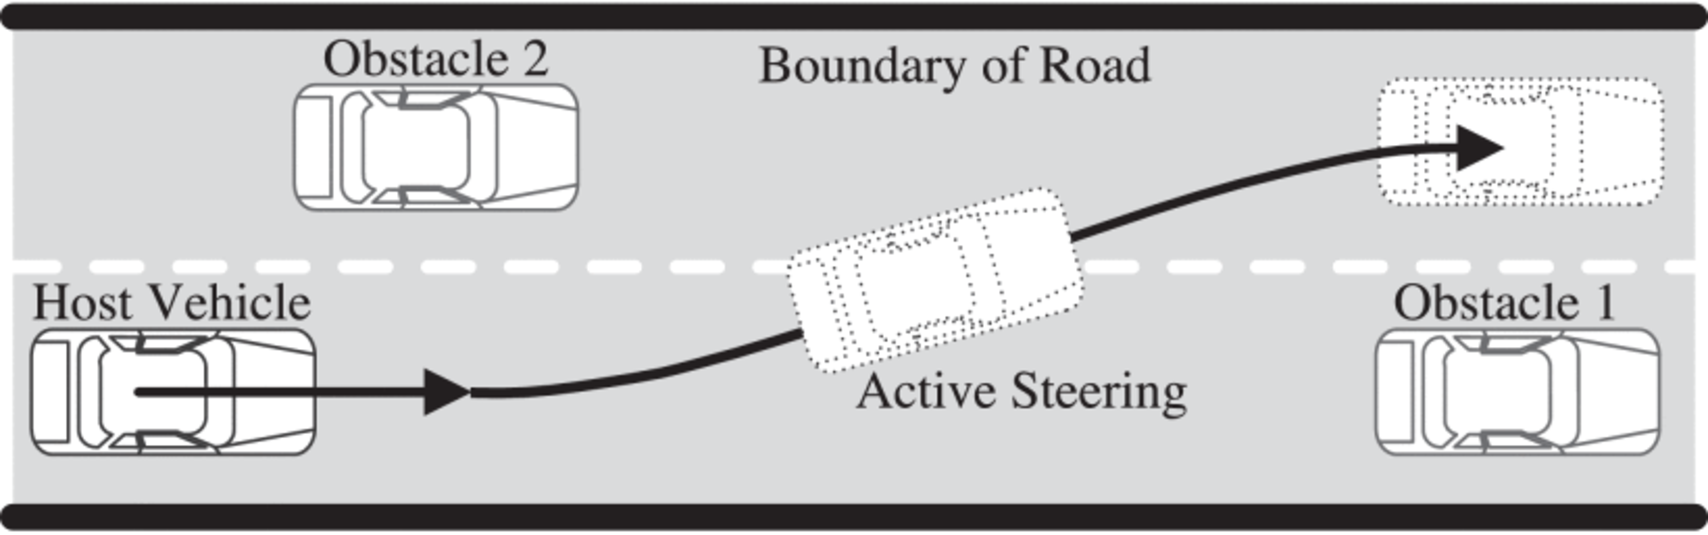
\includegraphics[width=1\columnwidth]{./figure/obstacleAvoidance.pdf}
	\caption{Problem description of collision avoidance on road.}
	\label{fig:obstacleAvoidance}
\end{figure}

The model used in this paper should take into account the kinematic and dynamic aspects of the vehicle. Here, we present a non linear mathematical model of a vehicle used for the development of a collision avoidance system.
The model has four states and two inputs:
\[ 
\textbf{x}=\begin{bmatrix}
   x&y&\theta&v 
  \end{bmatrix}^{T}
\qquad 
\textbf{u}=\begin{bmatrix}
T&\delta 
\end{bmatrix}^{T}
\]
where $(x,y)$ are the global coordinates of the center point of the car, $\theta$ is the heading angle of the car body with respect to the $x$-axis and $v$ is the speed of the car (positive). The manipulated variables are $T$ the throttle (positive when accelerating/negative when decelerating) and $\delta$ the steering angle ($0$ when aligned with car, counterclockwise positive).

The simple non-linear model to describe the dynamics of the ATLASCAR2 is the following
\begin{equation*}
	\label{eqn:dynamics_model_obstacle_avoidance}
	\left \{ \begin{array}{llll}
	\dot{x} = -v\sin(\theta)\cdot\theta+\cos(\theta)\cdot v\\
	\dot{y} = v\cos(\theta)\cdot\theta+\sin(\theta)\cdot v\\
	\dot{\theta} =(\tan(\delta)/C_L)\cdot v+ \bigg(v\bigg(\tan(\delta)^2+1\bigg)/C_L\bigg)\cdot \delta\\
	\dot{v} =0.5\cdot T
	\end{array} 
	\right .
\end{equation*}
where $C_L$ is the car length. The state equations can be re-written in a more compact form as follows:
\begin{equation}
	\label{eqn:dynamics_ss_obstacle_avoidance_con}
	\begin{array}{ll}
	\dot{\textbf{x}} =A_c \textbf{x}+ B_c \textbf{u}\\
	\textbf{y} =C_c \textbf{x} + D_c \textbf{u}
	\end{array}
\end{equation}
where
\[ 
A_c=\begin{bmatrix}
0&0&-v\sin(\theta)&\cos(\theta)\\
0&0&v\cos(\theta)&\sin(\theta)\\
0&0&0&\tan(\delta)/C_L\\
0&0&0&0
\end{bmatrix},
\]
\[
B_c=\begin{bmatrix}
0&0\\
0&0\\
0&v\bigg(\tan(\delta)^2+1\bigg)/C_L\\
0.5&0
\end{bmatrix},
\]
\[
C_c=\begin{bmatrix}
1&0&0&0\\
0&1&0&0\\
0&0&1&0\\
0&0&0&1
\end{bmatrix} = \textbf{I}_4, 
\qquad
D_c=\begin{bmatrix}
0&0\\
0&0\\
0&0\\
0&0
\end{bmatrix} = \textbf{0}_{4\times2}. 
\]
The system to be controlled is usually modeled by a discrete state-space model in the MPC literature. Therefore, (\ref{eqn:dynamics_ss_obstacle_avoidance_con})
is transformed into a discrete state-space model to be used by the model predictive controller:
\begin{equation}
\label{eqn:dynamics_ss_obstacle_avoidance_dis}
	\begin{array}{rr}
	{\textbf{x}}(k+1) =A_d \textbf{x}(k)+ B_d \textbf{u}(k)\\
	\textbf{y}(k) =C_d \textbf{x}(k) + D_d \textbf{u}(k)
	\end{array}
\end{equation}
where $A_d$ and $B d$ are the state and control matrices for the discrete state-space equation, respectively, which can be calculated with the Euler method as
\[
A_d = e^{A_cT_s},\qquad B_d = \int_{kT_s}^{(k+1)T_s} e^{A_c[(k+1)T_s-\eta]}B_c d\eta
\]
where $T_s$ is the sampling interval for the discrete state-space model. The matrices $C_d$ and $D_d$ are equivalent to those in the continuous case. For simplicity, we assume that all the states are measurable and the ATLASCAR2 drives east with a constant speed at the nominal operating point. In the scenario we are going to consider, the road is straight and our vehicle stays in the middle of the center lane when not passing. Without losing generality, the ATLASCAR2 passes an obstacle both to the right and to the left lane depending on where it is placed on the road. We create also a safe zone around the obstacles so that the vehicle does not get too close the osbtacle when passing it.

\subsection{Design of Adaptive Model Predictive Control}

We designed a model predictive controller that can make the ATLASCAR2 mantain a desired velocity and stay in the middle of center lane. We used an Adaptive MPC controller because it handles the nonlinear vehicle dynamics more effectively than a traditional MPC controller in fact the latter uses a constant plant model, however, the former allows us to provide a new plant model at each control interval. Because the new model describes the plant dynamics more accurately at the new operating condition, an adaptive MPC controller performs better than a traditional MPC controller. In practice at each control interval, the adaptive MPC controller updates the plant model and the nominal conditions. Once updated, the model and the conditions remain constant over the prediction horizon. At the beginning, we specified the constraints for the manipulated variables: to prevent the ATLASCAR2 from accelerating or decelerating too quickly, we added an hard constraint on the throttle rate of change and another one on the steering angle rate of change. We used an approach that takes advantage of the ability of MPC to handle constraint explicitly. When an obstacle is detected, it defines an area on the road (in terms of constraints) that the ATLASCAR2 must not enter during the prediction horizon. At the next control interval the area is redefined based on the new positions of the vehicle and the obstacle until passing is completed.
To define the area to avoid, we used the following mixed Input/Output constraints:
\begin{equation*}
	\label{eqn:mixed_IO_constraints}
	E\textbf{u}+F\textbf{y}\leq G
\end{equation*}
where $\textbf{u}$ and $\textbf{y}$ are respectively the manipulated variable vector and the output variable vector, while $E,F,G$ are the matrices that can be updated when the controller is running:
\begin{itemize}
	\item the first constraint is an upper bound on the $y$-coordinate (right boundary of the road);
	\item the second constraint is a lower bound on the $y$-coordinate (left boundary of the road);
	\item the third constraint is for the obstacle avoidance; even though no obstacle is detected at the nominal condition, we must add this fake constraint here because we cannot change the dimensions of the constraint matrices at run time (it has the same form as the second one).
\end{itemize}
The matrices for the above inequality are the following:
\[
E= 
\begin{bmatrix}
0&0\\
0&0\\
0&0\\
0&0
\end{bmatrix},
\quad
F=\begin{bmatrix}
0&1&0&0\\
0&-1&0&0\\
cS&-1&0&0
\end{bmatrix},\quad
G=
\begin{bmatrix}
W/2\\W/2\\-cI
\end{bmatrix}
\]
where $W$ is the width of the road and $cI$ and $cS$ are the required parameters such that the ATLASCAR2 must be above the line formed from the vehicle to safe zone corner for left/right passing.

\subsection{Simulation Results}
In this first simulation we assumed that the road is straight and has 3 lanes each of 4 meters wide. Moreover the ATLASCAR2 drives in the middle of the center lane when not passing and in this case the vehicle passes an obstacle only from the right lane (the same simulation can be launched so that the car goes over to the left fast lane).
\begin{figure}[!h]
	\centering
	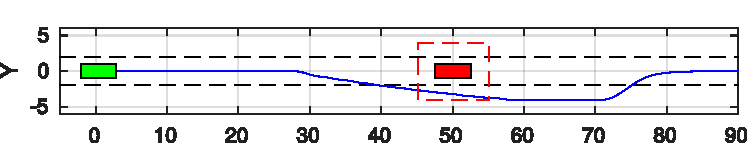
\includegraphics[width=1\columnwidth]{../../MATLAB/one_obstacle_right_overtaking/figure/overtaking_paper/overtaking_start.pdf}
	\label{fig:obstacleAvoidance_start}
\end{figure}
\vspace{-3em}
\begin{figure}[!h]
	\centering
	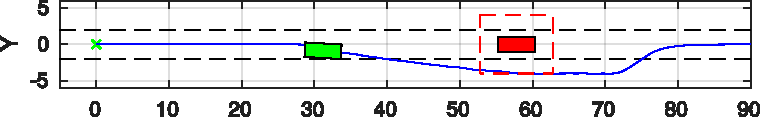
\includegraphics[width=1\columnwidth]{../../MATLAB/one_obstacle_right_overtaking/figure/overtaking_paper/overtaking_middle.pdf}
	\label{fig:obstacleAvoidance_middle}
\end{figure}
\vspace{-3em}
\begin{figure}[!h]
	\centering
	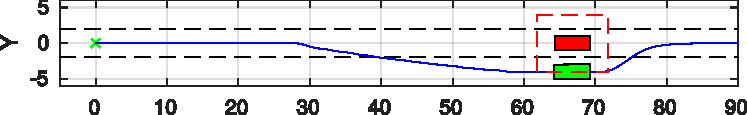
\includegraphics[width=1\columnwidth]{../../MATLAB/one_obstacle_right_overtaking/figure/overtaking_paper/overtaking_middle_end.pdf}
	\label{fig:obstacleAvoidance_middle_end}
\end{figure}
\vspace{-3em}
\begin{figure}[!h]
	\centering
	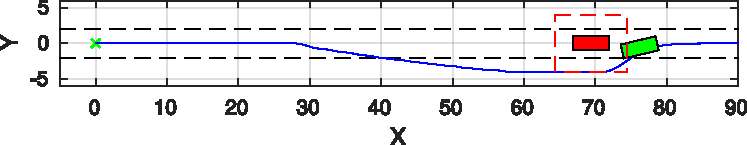
\includegraphics[width=1\columnwidth]{../../MATLAB/one_obstacle_right_overtaking/figure/overtaking_paper/overtaking_end.pdf}
	\label{fig:obstacleAvoidance_end}
	\vspace{-1.2em}
	\caption{Simulation of right overtaking with one moving obstacle}
\end{figure}

Subsequently, additional obstacles were added to make the scenario more complex. The vehicle is capable of overcoming the obstacles to the right or left depending on their position with respect to the road. We also hypothesized that the obstacles move at a different speed but that they are initially at a common distance. In case two obstacles are too close during the simulation and their distance is less than the detection range, the ATLASCAR2 perceives the objects as a single entity and adapts to the situation.

\begin{figure}[!h]
	\centering
	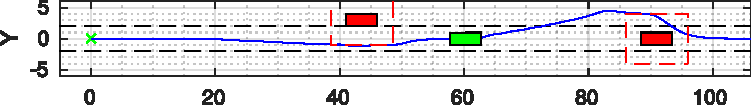
\includegraphics[width=1\columnwidth]{../../MATLAB/random_N_obstacles/figure/overtaking_random_2.pdf}
	\label{fig:obstacleAvoidance_random_2}
	\vspace{-1.3em}
\end{figure}
\begin{figure}[!h]
	\centering
	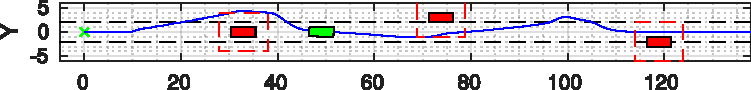
\includegraphics[width=1\columnwidth]{../../MATLAB/random_N_obstacles/figure/overtaking_random.pdf}
	\label{fig:obstacleAvoidance_random}
	\vspace{-1.3em}
\end{figure}
\begin{figure}[!h]
	\centering
	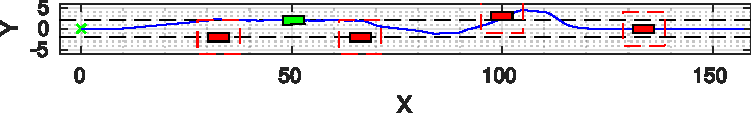
\includegraphics[width=1\columnwidth]{../../MATLAB/random_N_obstacles/figure/overtaking_random_1.pdf}
	\label{fig:obstacleAvoidance_random_1}
	\vspace{-1.2em}
	\caption{Simulations of overtaking with $N = 2,3,4$ moving obstacles}
\end{figure}

















\section{Lane Following}
\subsection{Problem Formulation}
A lane-following system is a control system that keeps the vehicle traveling along the centerline of a highway lane, while maintaining a user-set velocity. The lane-following scenario is depicted in the following figure:
\begin{figure}[!h]
	\centering
	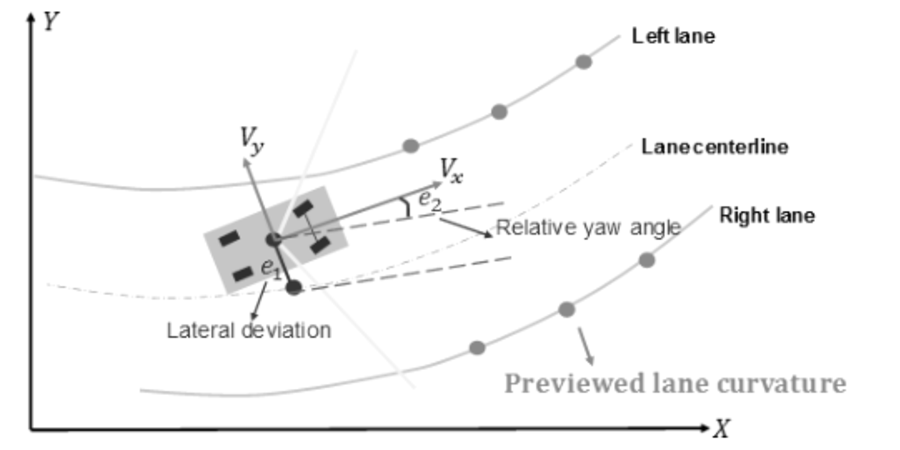
\includegraphics[width=1\columnwidth]{./figure/laneFollowing.pdf}
	\caption{Problem description of a lane following system.}
	\label{fig:laneFollowing}
\end{figure}

In a classic lane keeping assist, it is assumed that the longitudinal velocity is constant. This restriction is relaxed in this model because the longitudinal acceleration varies in this MIMO control system. This lane-following system manipulates both the longitudinal acceleration and the front steering angle of the vehicle to keep the lateral deviation and the relative yaw angle small and the longitudinal velocity close to a driver set velocity. If these two goals cannot be met at the same moment, the system tries to balance them. The model that we are considering, contains a lot of parameters. The first fundamental block describes the vehicle dynamics: we have applied the bicycle model of lateral vehicle dynamics and approximate the longitudinal dynamics using a time constant:
\subsubsection{Longitudinal dynamics}
\begin{equation}
	\label{eqn:longi_dynamics_simple_model}
	G(s)=\frac{1}{\tau s^2+s} \quad \text{where $\tau$ is a time constant}
\end{equation}

\subsubsection{Lateral dynamics}
Local function: we have a continuous vehicle lateral model from parameters
\begin{equation}
\label{eqn:lateral_dynamics_simple_model}
\begin{array}{ll}
\dot{\textbf{x}}_{\text{lat}} =A_g \textbf{x}_{\text{lat}}+ B_g \textbf{u}_{\text{lat}}\\
\textbf{y}_{\text{lat}} =C_g \textbf{x}_{\text{lat}} + D_g \textbf{u}_{\text{lat}}
\end{array}
\end{equation}
where the input is the steering angle in radians, and the outputs are the lateral velocity in meters per second and yaw angle rate in radians per second:
\begin{equation*}
\textbf{x}_{\text{lat}} = \begin{bmatrix}
V_y&\dot{\psi}
\end{bmatrix}^T
\qquad
\textbf{u}_{\text{lat}} = \delta
\end{equation*}
and
\[ 
A_g=\begin{bmatrix}
-\frac{2C_F+2C_R}{mV_x}&-\frac{2C_Fl_F-2C_Rl_R}{mV_x} - V_x\\
-\frac{2C_Fl_F-2C_Rl_R}{I_ZV_x}&-\frac{2C_Fl_F^2+2C_Rl_R^2}{I_ZV_x}
\end{bmatrix},
\]
\[
B_g=\begin{bmatrix}
2C_F/m\\
2C_Fl_F/I_Z
\end{bmatrix},
\quad
C_g=\textbf{I}_2, 
\quad
D_g=\textbf{0}_{2\times1}.
\]
The parameters in the previous matrices are:
\begin{itemize}
	\item $V_x$ is the longitudinal velocity of the car;	
	\item $m$ is the total mass parameter; 
	\item $I_Z$ is the yaw moment of inertia parameter;
	\item $l_F$ and $l_R$ are the longitudinal distances from center of gravity to front and rear tires parameters;
	\item $C_F$ and $C_R$ are the cornering stiffnesses of front and rear tires parameters.
\end{itemize}
The goal for the driver steering model is to keep the vehicle in its lane and follow the curved road by controlling the front steering angle . This goal is achieved by driving the yaw angle error $e_2 = \psi -\psi_{\text{des}}$ and lateral displacement error $e_1$ to zero ($\dot{e}_1 = V_xe_2+V_y$). We can incorporate these two paramenters in the augmented model:
\begin{equation}
\label{eqn:lateral_dynamics_augmented_model}
\begin{array}{ll}
\dot{\textbf{x}}_{\text{aug}} =A_a \textbf{x}_{\text{aug}}+ B_a \textbf{u}_{\text{aug}}\\
\textbf{y}_{\text{aug}} =C_a \textbf{x}_{\text{aug}} + D_a \textbf{u}_{\text{aug}}
\end{array}
\end{equation}
where
\begin{equation*}
\textbf{x}_{\text{aug}} = \begin{bmatrix}
V_y&\dot{\psi}&e_1&e_2
\end{bmatrix}^T,
\qquad
\textbf{u}_{\text{aug}} = 
\begin{bmatrix}
\delta&\dot{\psi}_{\text{des}}
\end{bmatrix}^T
\end{equation*}
and
\[ 
A_a=\begin{bmatrix}
A_g&\textbf{0}_{2\times2}\\
\textbf{I}_2&\begin{matrix}
0&V_x\\
0&0
\end{matrix}
\end{bmatrix},
\quad
B_a=\begin{bmatrix}
B_g&\textbf{0}_{2\times1}\\
0&0\\
0&-1
\end{bmatrix},
\]
\[
C_a=\begin{bmatrix}
\textbf{0}_{2\times2}&\textbf{I}_2
\end{bmatrix}, 
\quad
D_a=
\textbf{0}_{2\times2}. 
\]
Combining (\ref{eqn:longi_dynamics_simple_model}) with (\ref{eqn:lateral_dynamics_augmented_model}) yields the state-space model that characterizes the model predictive controller:
\begin{equation}
\label{eqn:full_dynamics_model}
\begin{array}{ll}
\dot{\textbf{x}}_{\text{tot}} =A_f \textbf{x}_{\text{tot}}+ B_f \textbf{u}_{\text{tot}}\\
\textbf{y}_{\text{tot}} =C_f \textbf{x}_{\text{tot}} + D_f \textbf{u}_{\text{tot}}
\end{array}
\end{equation}
where
\begin{equation*}
\textbf{x}_{\text{tot}} = \begin{bmatrix}
V_x\\\dot{V}_x\\V_y\\\dot{\psi}\\e_1\\e_2
\end{bmatrix},
\qquad
\textbf{u}_{\text{tot}} = 
\begin{bmatrix}
a\\\delta\\\dot{\psi}_{\text{des}}
\end{bmatrix}
\end{equation*}
and


\[ 
A_f=\begin{bmatrix}
\begin{matrix}-2&0\\1&0\end{matrix}&\textbf{0}_{2\times4}\\
\textbf{0}_{4\times2}&A_a
\end{bmatrix},
\quad
B_f=\begin{bmatrix}\begin{matrix}2\\0\end{matrix}&\textbf{0}_{2\times2}\\
\textbf{0}_{4\times1}&B_a
\end{bmatrix},
\]
\[
C_f=\begin{bmatrix}
\begin{matrix}0&1\end{matrix}&\textbf{0}_{1\times4}\\
\textbf{0}_{2\times2}&C_a
\end{bmatrix}, 
\quad
D_f=\textbf{0}_{3\times3}. 
\]

However the system to be controlled is usually modeled by a discrete state-space model:
\begin{equation*}
\label{eqn:full_dynamics_model_disc}
\begin{array}{rr}
{\textbf{x}}_{\text{tot}}(k+1) =A \textbf{x}_{\text{tot}}(k)+ B \textbf{u}_{\text{tot}}(k)\\
\textbf{y}_{\text{tot}}(k) =C\textbf{x}_{\text{tot}}(k) + D \textbf{u}_{\text{tot}}(k)
\end{array}
\end{equation*}
where $A$ and $B$ are the state and control matrices for the discrete state-space equation, respectively, which can be calculated, also in this case, with the Euler method as:
\[
A = e^{A_fT_s},\qquad B = \int_{kT_s}^{(k+1)T_s} e^{A_f[(k+1)T_s-\eta]}B_f d\eta
\]
where $T_s$ is the sampling interval for the discrete state-space model. The matrices $C$ and $D$ are equivalent to those in the continuous case.

\subsection{Design of Adaptive Model Predictive Control}
We created an Adaptive MPC controller with a prediction model that has six states, three outputs (longitudinal velocity, lateral deviation, relative yaw angle), and two inputs. The model has two manipulated signals: acceleration and steering. The product of the road curvature and the longitudinal velocity is modeled as a measured disturbance. We have set the constraints for manipulated variables and the scale factors. Moreover we have specified the weights in the standard MPC cost function. The third output, yaw angle, is allowed to float because there are only two manipulated variables to make it a square system. In this controller, there is no steady-state error in the yaw angle as long as the second output, lateral deviation, reaches 0 at steady state. Finally we have also penalized acceleration change more for smooth driving experience. This controller uses a linear model for the vehicle dynamics and updates the model online as the longitudinal velocity varies.

\subsection{Simulation Results}
The proposed adaptive MPC algorithm is designed in the MATLAB/Simulink and validated through simulation. The objective of this
test is to evaluate the behavior of the proposed control strategy in critical situations. Fig.\ref{fig:reference_laneFollowing} and Fig.\ref{fig:curvature_laneFollowing} show the desired path that the car must follow and its curvature.
\begin{figure}[!h]
	\centering
	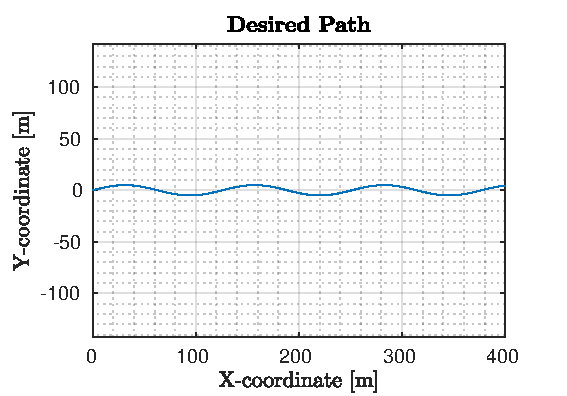
\includegraphics[width=1\columnwidth]{../../MATLAB/lane_following/figure/Reference.pdf}
	\caption{Desired path of the ATLASCAR2.}
	\label{fig:reference_laneFollowing}
\end{figure}
\begin{figure}[!h]
	\centering
	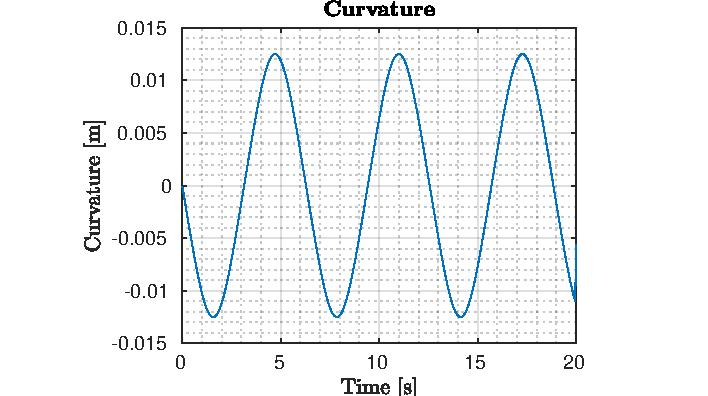
\includegraphics[width=1\columnwidth]{../../MATLAB/lane_following/figure/Curvature.pdf}
	\caption{Desired curvature.}
	\label{fig:curvature_laneFollowing}
\end{figure}

Moreover the following figures show the trend of the main parameters confirming that the control strategy used allows the vehicle to follow the path. In particular we simulated also a small error in the sensor dynamics in order to make the simulation more realistic: we added a 3 percent error to the longitudinal velocity and this is evident from the small noise in the graphs of the steering angle and the lateral deviation.

\begin{figure}[!h]
	\centering
	\hspace*{-0.5in}
	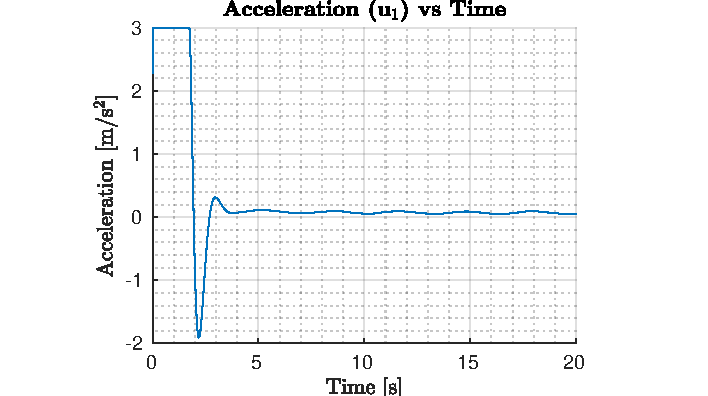
\includegraphics[width=1.29\columnwidth]{../../MATLAB/lane_following/figure/AccelerationVsTime.pdf}
	\caption{Acceleration $u_1$ with respect to time.}
	\label{fig:acceleration_laneFollowing}
\end{figure}
\begin{figure}[!h]
	\centering
	\hspace*{-0.5in}
	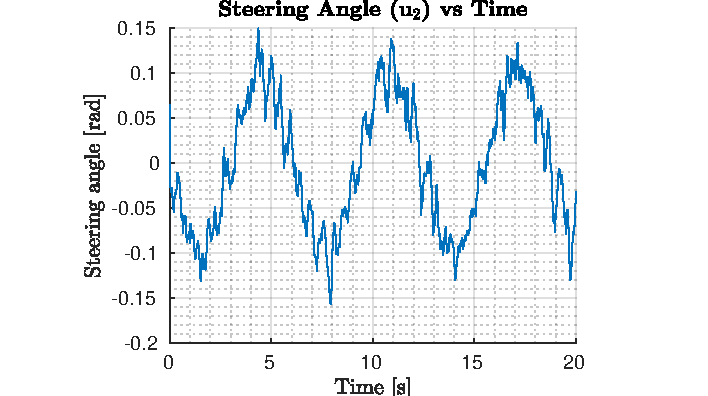
\includegraphics[width=1.29\columnwidth]{../../MATLAB/lane_following/figure/SteeringAngleVsTime.pdf}
	\caption{Steering angle $u_2$ with respect to time.}
	\label{fig:steering_laneFollowing}
\end{figure}
\begin{figure}[!h]
	\centering
	\hspace*{-0.5in}
	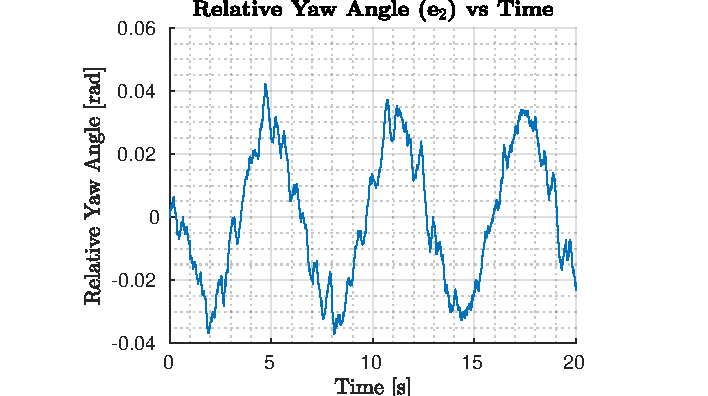
\includegraphics[width=1.29\columnwidth]{../../MATLAB/lane_following/figure/RelativeYawAngleVsTime.pdf}
	\caption{Relative yaw angle $e_2$ with respect to time.}
	\label{fig:relative_yaw_angle_laneFollowing}
\end{figure}
\begin{figure}[!h]
	\centering
	\hspace*{-0.5in}
	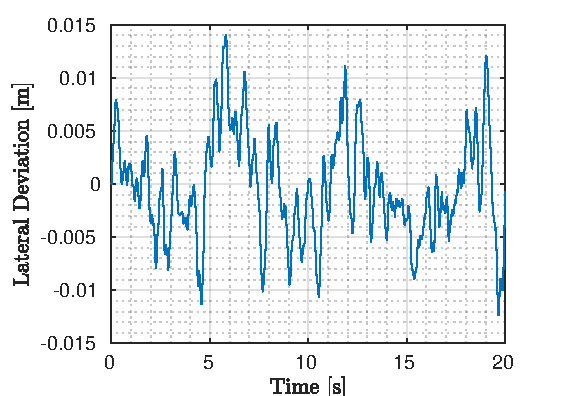
\includegraphics[width=1.29\columnwidth]{../../MATLAB/lane_following/figure/LateralDeviationVsTime.pdf}
	\caption{Lateral deviation $e_1$ with respect to time.}
	\label{fig:lateral_deviation_laneFollowing}
\end{figure}
Fig.{\ref{fig:longitudinal_velocity_laneFollowing}} shows the evolution of the vehicle longitudinal velocity. At the start of the simulation, this velocity is equal to the initial condition for longitudinal velocity parameter. At run time, this velocity is equal to the Longitudinal velocity input signal. We can note that $V_x$ reaches the predefined value of $20$ meters for second and then it stabilizes near the cruising speed because it continues to vary the steering angle to adapt to the path to be followed.
\begin{figure}[!h]
	\centering
	\hspace*{-0.5in}
	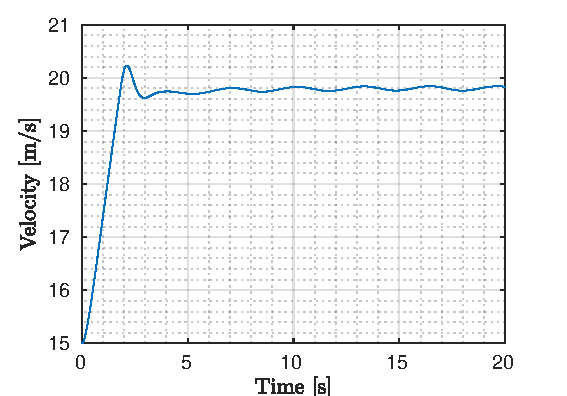
\includegraphics[width=1.29\columnwidth]{../../MATLAB/lane_following/figure/LongitudinalVelocityVsTime.pdf}
	\caption{Longitudinal velocity $V_x$ with respect to time.}
	\label{fig:longitudinal_velocity_laneFollowing}
\end{figure}


\begin{figure*}[!h]
	\centering
	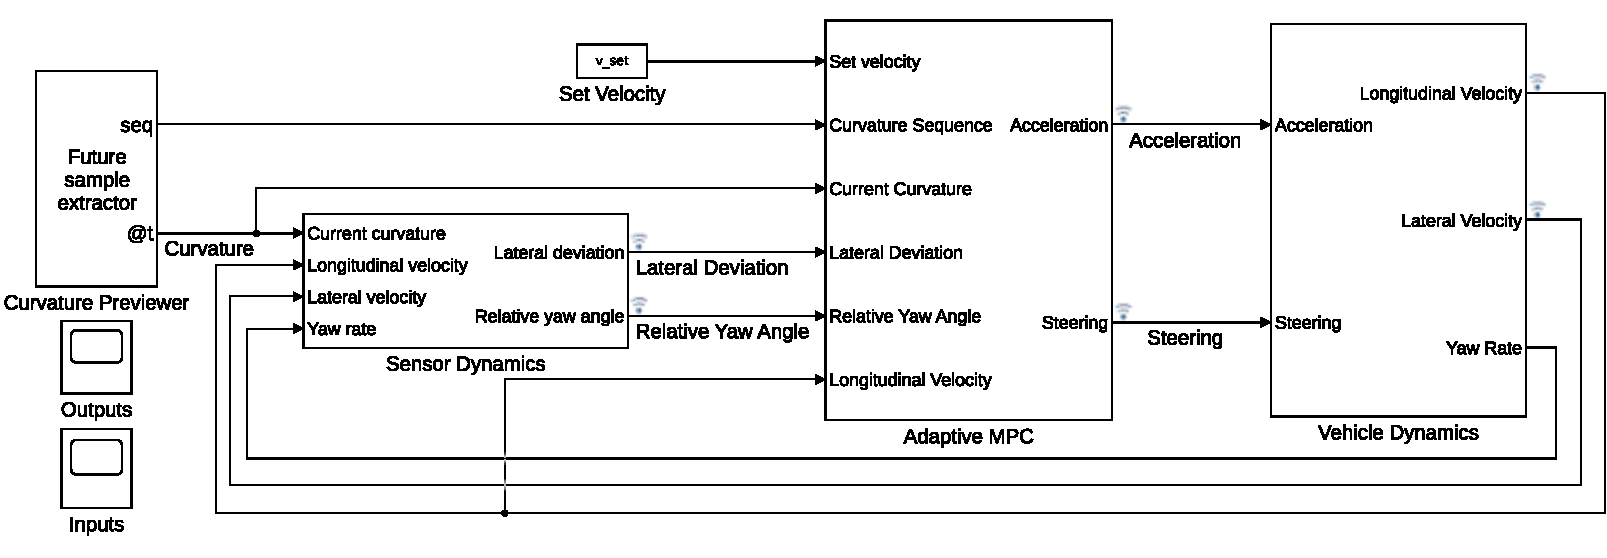
\includegraphics[width=\textwidth]{./figure/lane_following_AMPC.pdf}
	\caption{Overall procedure scheme lane following.}
	\label{fig:scheme_lane_following}
\end{figure*}


\section{Conclusions and Future Work}
In this work we proposed two advanced methods for the ATLASCAR2 based on adaptive Model Predictive Control. In the first case we analyzed an obstacle avoidance system that moves the vehicle around different moving obstacles in the lane using throttle and steering angle. This system updates both the predictive model and the mixed input/output constraints at each control interval. Instead, in the second scenario  we have developed a lane following system that keeps the ATLASCAR2 traveling along the centerline of the lanes on the road by adjusting the front steering angle of the car. The flexibility of the concepts used in these methods allows a multitude of refinements and extensions to this project. For example the next possible work could be to combine the two previous control strategies in a way that they can operate simultaneously. Moreover the final method could be tested in a real autonomous driving scenario.








\begin{thebibliography}{00}
	\bibitem{MMPC}J. Ji, A. Khajepour, W. W. Melek and Y. Huang, "Path Planning and Tracking for Vehicle Collision Avoidance Based on Model Predictive Control With Multiconstraints," in IEEE Transactions on Vehicular Technology, vol. 66, no. 2, pp. 952-964, Feb. 2017.
	
	\bibitem{onlineMPC}M. Werling and D. Liccardo, "Automatic collision avoidance using model-predictive online optimization," 2012 IEEE 51st IEEE Conference on Decision and Control (CDC), Maui, HI, 2012, pp. 6309-6314.
	
	\bibitem{swarms}Wei Xi and J. S. Baras, "MPC based motion control of car-like vehicle swarms," 2007 Mediterranean Conference on Control \& Automation, Athens, 2007, pp. 1-6.
	
	\bibitem{autoMPC}J. V. Frasch et al., "An auto-generated nonlinear MPC algorithm for real-time obstacle avoidance of ground vehicles," 2013 European Control Conference (ECC), Zurich, 2013, pp. 4136-4141.
	
	\bibitem{safety}T. Xu and H. Yuan, "Autonomous vehicle active safety system based on path planning and predictive control," 2016 35th Chinese Control Conference (CCC), Chengdu, 2016, pp. 8889-8895.
	
	\bibitem{matsumoto}N. Wada and T. Matsumoto, "Driver assistance for collision avoidance by constrained MPC," 2017 56th Annual Conference of the Society of Instrument and Control Engineers of Japan (SICE), Kanazawa, 2017, pp. 90-93.
	
	\bibitem{fuzzyMPC}Y. Nishio, K. Nonaka and K. Sekiguchi, "Moving obstacle avoidance control by fuzzy potential method and model predictive control," 2017 11th Asian Control Conference (ASCC), Gold Coast, QLD, 2017, pp. 1298-1303.
	
	\bibitem{NONMPC}Yu, S., Li, X., Chen, H. and Allgöwer, F. (2015), "Nonlinear model predictive control for path following problems". Int. J. Robust Nonlinear Control, 25: 1168–1182. 
	
	\bibitem{matPDF}A. Bemporad, M. Morafi, and N. Ricker, Model Predictive Control Toolbox User’s Guide, The MathWorks, Inc.,
	
		\url{https://www.mathworks.com/help/pdf_doc/mpc/mpc_ug.pdf}
		
	\bibitem{theory}J. Rawlings, D. Mayne (2010), "Model Predictive Control: Theory and Design", Nob Hill Publishing.	
\end{thebibliography}


\end{document}